\chapter{Межмодульный анализ} \label{chapt3}

Межпроцедурный анализ можно разделить на две категории в зависимости от области поиска определений вызываемых функций: на внутримодульный и межмодульный. Внутримодульный анализ подразумевает поиск доступных определений функций только в анализируемом модуле трансляции, тогда как в случае межмодульного анализа поиск определений может производиться и в других модулях трансляции. Очевидно, что в случае внутримодульного анализа анализатору может быть доступна лишь часть пользовательских определений функций, несмотря на потенциальную доступность исходного  кода моделируемых функций. При межмодульном анализе потенциально недоступными являются лишь библиотечные функции с недоступным исходным кодом.

Межмодульный анализ позволяет находить различные классы дефектов программного кода, не обнаруживаемые при внутримодульном анализе или труднообнаружимые с его помощью. К таким дефектам относятся ошибки интеграции модулей и подсистем программы или программного комплекса, некорректное использование программных интерфейсов (API). Межмодульный анализ становится особенно полезным для языков программирования, допускающих раздельную компиляцию исходных файлов, поскольку в этом случае информация о программе, содержащаяся в одном исходном файле, становится крайне ограниченной и затрагивает лишь малую часть программного проекта. В число таких языков входят C и C++, исходные файлы которых обычно сначала компилируются в объектный код, и уже затем результирующие модули компонуются между собой, что позволяет получить всю информацию о программе лишь на поздних этапах её построения. Таким образом, проблема межмодульного анализа  должна быть решена любым анализатором, выполняющим межпроцедурный анализ программ, разработанных с использованием данного языка.

Различные инструменты анализа кода реализуют межмодульный анализ по-разному. В случае динамического анализа анализируются не определения функций, а сгенерированный код: объектный код или промежуточное представление. В этом случае код вызываемых функций непосредственно становится доступным анализатору или в момент загрузки анализируемого модуля, или в процессе выполнения программы при загрузке подгружаемых модулей.

Большинство статических анализаторов, имеющих возможность межмодульного анализа, используют в качестве входных данных анализа промежуточное представление. Так, статический анализатор Svace \cite{svace} использует для анализа байт-код LLVM, Coverity SAVE \cite{coverity}~--- компилятор Edison Design Group, и строят глобальный граф вызовов анализируемого проекта, производя разбор байт-кода, предварительно сгенерированного из исходных файлов проекта. Clang Static Analyzer, в отличие от многих других инструментов анализа исходного кода методом символьного выполнения, использует в качестве входных данных не промежуточное представление или объектный код, а непосредственно исходные файлы. Одной из основных причин этого является удобная и удачно спроектированная реализация абстрактного синтаксического дерева, в котором представлена вся информация о программе без каких-либо предварительных оптимизаций или потерь информации. Это обстоятельство требует применения иных подходов к межмодульному анализу, нежели в Coverity SAVE или Svace. В связи с этим в данной работе для проведения межмодульного анализа с использованием фреймворка Clang Static Analyzer предлагается  выполнять слияние синтаксических деревьев различных файлов, связанных вызовами функций.

В результате проведённого исследования была разработана архитектура анализатора, позволяющего производить межмодульный анализ программы на языках C и C++ и использующем для анализа непосредственно исходный код программы. Разработанная схема межмодульного анализа интересна тем, что позволяет использовать различные алгоритмы межпроцедурного анализа, т.~е. как анализ методом встраивания, так и анализ методом резюме, без каких-либо дополнительных модификаций как самого алгоритма межпроцедурного анализа, так и проверяющих модулей. <<Прозрачный>> межмодульный анализ позволит в дальнейшем провести корректное сравнение различных алгоритмов межпроцедурного анализа при использовании межмодульного подхода. Данное сравнение представляет интерес, поскольку при использовании межмодульного анализа количество анализируемых путей внутри программы быстро растёт, что может представлять сложность при использовании межпроцедурного анализа.

\section{Реализация межмодульного анализа в статическом анализаторе, использующем для анализа непосредственно исходный код программы}

Единицей анализа в Clang Static Analyzer является транслируемый модуль, представляющий собой препроцессированный файл исходного кода. Однако для выполнения межмодульного анализа информации, содержащейся в одном транслируемом модуле, недостаточно. Необходимо знать расположение определений функций, необходимых для анализа других функций. Кроме того, необходимо знать не только имя и путь к файлу, где располагается определение функции. Для корректного построения импортируемого синтаксического дерева файла с исходным текстом необходимо знать, например, аргументы команды сборки файла, расположение включаемых файлов, использовавшихся для построения, и некоторую другую информацию.

Именно Clang Static Analyzer является целевым анализатором для реализации межмодульного анализа в данной работе, поскольку ранее автором был реализован ряд других проектов с использованием данного анализаторного фреймворка, и реализация межмодульного анализа является их завершающей частью. Кроме того, использование межмодульного анализа резко увеличивает количество требующих анализа путей программы и представляет интерес при сравнении производительности и качества межпроцедурного анализа методом встраивания и разработанного автором метода резюме. Таким образом, в данной работе рассматривается решение проблемы межмодульного анализа для случая использования анализатором непосредственно исходного кода программы.

Для решения проблемы определения местоположения анализируемых функций, в данной работе реализован трёхфазный анализ с сохранением промежуточных результатов в файлах в директории проекта. Таким образом, анализ разделяется на три фазы: фаза сборки, фаза предобработки данных и непосредственно сам анализ исходных кодов. На рисунке \ref{xtu-idef0} представлена схема взаимодействия инструментов, используемых на различных фазах анализа, в виде диаграммы IDEF0. На этой схеме модули, реализованные в данной работе полностью, обозначены белым цветом, а серым обозначены модули, существовавшие ранее и доработанные для использования при межмодульном анализе: \texttt{clang} является непосредственно статическим анализатором, использованным для реализации межмодульного анализа, а Perl-скрипт \texttt{ccc-analyzer} входит в состав вспомогательного пакета \texttt{scan-build} и служит для формирования командной строки запуска статического анализатора \texttt{clang} и его запуска.

\begin{figure}[h]
 \label{}
 \centering
 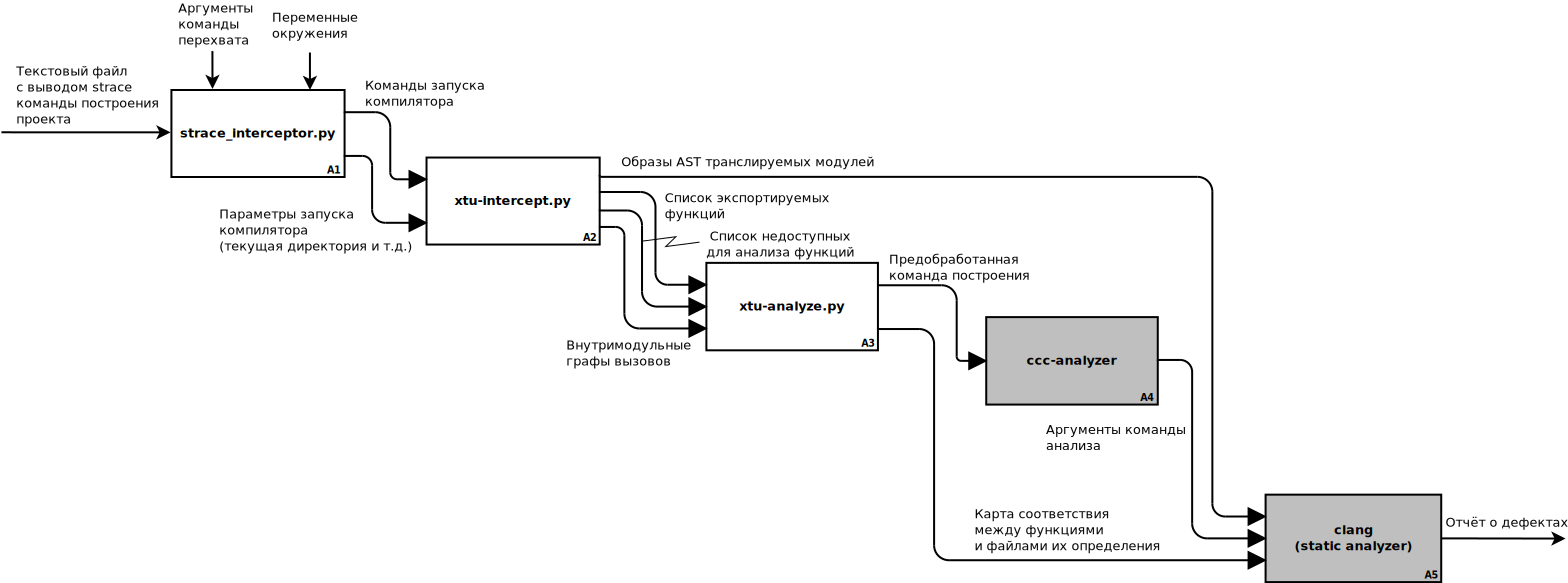
\includegraphics[width=\linewidth]{xtu-idef0}
 \caption{IDEF0-диаграмма взаимодействия разработанных программных инструментов при межмодульном анализе}\label{xtu-idef0}
\end{figure}


\section{Фаза сборки}

На фазе сборки специальный инструмент (\texttt{strace\_interceptor}), использующий программу \texttt{strace}, собирает информацию о транслируемых модулях, которые должны быть проанализированы. Программа \texttt{strace} является утилитой ОС Linux, задачей которой является трассировка указываемого процесса (и, опционально, его потомков) и вывод информации о системных вызовах трассируемых процессов в стандартный поток вывода. Инструмент \texttt{strace\_interceptor} реализован с использованием языка Python. Данный инструмент был разработан в рамках данной работы с целью поддержки различных систем сборки, в том числе, использующих сборку проекта в <<песочнице>>, без изменения сборочных конфигураций. В число поддерживаемых систем сборки входят Makefile, Open Build Service (OBS~--- при локальном построении проекта с использованием клиентского приложения \texttt{osc}) \cite{obs} и Git Build System (GBS) \cite{gbs}, причём поддерживается, в том числе, сборка в <<песочнице>> другой архитектуры с использованием эмуляторов (например, Qemu). Разработанный инструмент выполняет разбор вывода утилиты strace и использует информацию о системных вызовах \texttt{chroot()}, \texttt{chdir()}, \texttt{vfork()} и \texttt{execve()} для поиска вызовов компилятора и записывает текущую директорию, корневую директорию, команду сборки и переменные окружения в файл. Корневая директория отличается от стандартной (<</>>) в тех случаях, когда был выполнен вызов \texttt{chroot()}. Текущая директория задаётся относительно корневой. Задачей этого же инструмента является поиск директорий с включаемыми файлами, связанными с запускаемым при сборке компилятором. Затем для каждой обнаруженной команды сборки другой инструмент, использующий программный интерфейс (API) Clang (\texttt{clang-func-mapping}), записывает сигнатуры видимых извне (экспортируемых) определений функций данного модуля трансляции и сигнатуры используемых (импортируемых) функций, определения которых в данном модуле трансляции недоступны, в служебные файлы в директории проекта. Этот же инструмент для каждой обнаруженной функции строит локальный граф вызовов, который также сохраняется в служебный файл. На фазе сборки дополнительно создаются образы абстрактных синтаксических деревьев для всех модулей трансляции, что упрощает дальнейший импорт и позволяет избежать повторных вызовов компилятора для каждого импортируемого файла.

Необходимо учитывать целевую архитектуру сборки для каждого файла исходных кодов. Сборка одного и того же файла может выполняться одновременно для нескольких архитектур в пределах одной сессии сборки. Это особенно актуально при использовании в качестве основных тестовых комплексов мультиплатформенных систем с эмуляторами в своём составе. Например, в случае ОС Android, некоторые файлы строятся как для хост-архитектуры (на которой запускается эмулятор), так и для целевой архитектуры (эмулируемой). Это значит, что для корректного импорта определения функции необходимо различать целевые тройки (target triple) цели сборки файла. Нельзя использовать определения функций из файлов, предназначенных для разных архитектур, по следующим причинам.

\begin{enumerate}
 \item Определения функций для различных архитектур могут не совпадать непосредственно, в отношении текстового сравнения компилируемого исходного кода. Это возможно, поскольку для разных архитектур могут быть использованы различные фрагменты кода в директивах условной компиляции.
 \item По тем же причинам для разных архитектур может не совпадать окружение функции: определения используемых типов, зависимые определения. Кроме того, для разных архитектур могут использоваться различные включаемые файлы.
 \item Даже при совпадении окружения и текста функций, для различных архитектур могут не совпадать определения основных типов. Так, тип char является по умолчанию знаковым (\texttt{signed char}) для платформы x86 и беззнаковым (\texttt{unsigned char}) для платформы ARM.
\end{enumerate}

Кроме того, существует ещё одна проблема. Один и тот же модуль трансляции может собираться несколько раз в рамках сборки для одной архитектуры. При этом также могут быть использованы различные директивы препроцессора и включаемые файлы, что может привести к потенциальной несовместимости импортируемого и импортирующего синтаксических деревьев.

Все вышеперечисленные факторы означают, что выбирать модуль трансляции для импорта определения функции надо крайне осторожно. Для решения этой проблемы можно предложить несколько способов. В настоящей работе было использовано менее общее, но более простое в реализации решение. Для такого приближённого учёта архитектур достаточно знать, объектные модули каких архитектур могут компоноваться друг с другом. Например, объектные модули, скомпонованные для архитектур <<arm>> и <<thumb>> могут быть использованы для компоновки в один объектный файл при использовании определённых опций компилятора, тогда как <<arm>> и <<x86>> не могут. После построения такой матрицы, можно различать определения функций по тройке <путь к файлу, сигнатура функции, целевая архитектура>, и использовать эту тройку для выбора нужного определения функции и его импорта. Этот подход, хотя и прост в реализации, однако, не решает проблемы, связанной с использованием различных опций компилятора для одной и той же архитектуры, поскольку выбираться будет только один файл. Другим, и более общим решением видится поддержка <<дерева сборки>>. В этом случае на фазе сборки отслеживается полное дерево компиляции, ассемблирования и компоновки (и, возможно, сборки в бинарный образ) для объектных файлов верхнего уровня. Это позволяет точно определить, какая функция из какого исходного файла должна быть использована для моделирования межфайлового вызова. Кроме того, это частично решает проблему модулей трансляции, которые собираются несколько раз в рамках сборки для одной архитектуры, поскольку для каждой из сборок становится известен высокоуровневый модуль, для которого она производится. Вместе с тем, этот подход имеет и некоторые проблемы. Во-первых, при его использовании необходимо отслеживать не только вызовы компилятора, но также вызовы ассемблера и компоновщика. Во-вторых, некоторые файлы собираются очень часто. Так, при построении образа ОС Android встречаются файлы, которые собираются 38 раз. Это может означать необходимость множественного повторного анализа уже проанализированных модулей трансляции. Таким образом, выбор между этими вариантами нельзя назвать однозначным, поскольку у каждого из них есть свои преимущества и недостатки.

\section{Фаза предобработки данных}

Фаза предобработки данных необходима для обработки служебной информации, собранной на фазе сборки. На этой фазе строится соответствие между сигнатурами импортируемых функций. Как только соответствие становится известным, мы можем построить глобальный граф вызовов с использованием локальных графов вызовов, которые были сгенерированы на предыдущей фазе. Каждый узел графа вызовов, таким образом, представляет собой тройку <файл определения, сигнатура функции, архитектура>. После этого выполняется топологическая сортировка построенного глобального графа вызовов. Сначала анализируются функции верхнего уровня, затем функции, участвующие в рекурсивных цепочках вызовов, а затем~--- функции нижнего уровня. При этом сортируются не сами функции, а файлы, их содержащие, поскольку анализ отдельных функций из файла означает многократную загрузку одних и тех же файлов. И, наконец, после фазы предобработки данных запускается анализ модулей трансляции в топологическом порядке глобального графа вызовов.

Топологическая сортировка улучшает производительность, поскольку анализ производится по одному транслируемому модулю. Так как импорт определений функций и создание их резюме производится при первом моделировании вызова, выгоднее производить анализ, начиная с верхних уровней иерархии к нижним, что позволяет избежать повторных анализов одной и той же функции. В данной разработке используется список сигнатур проанализированных функций, чтобы исключить их повторный анализ вне контекста вызовов, т.~е., если анализ функции был произведён в контексте вызова, повторный анализ производиться не будет. Это объясняется тем, что анализ функции при сборке резюме не отличается от отдельного анализа функции, поэтому нет причин производить анализ функции вне контекста, если она уже была проанализирована для сбора резюме.

\section{Фаза анализа. Слияние синтаксических деревьев}

На вход фазы анализа поступает файл с упорядоченным набором файлов для анализа. Все эти файлы добавляются в очередь анализа в порядке следования в исходном файле, после чего полученная очередь начинает обрабатываться пулом рабочих процессов анализатора. Данная схема позволяет осуществлять анализ с очень высокой степенью параллелизма, т.~к. различные процессы не используют разделяемых ресурсов, и её производительность линейно растёт с увеличением количества процессоров (проверена масштабируемость до 32-х процессоров включительно). Каждый анализатор из пула анализирует свой транслируемый модуль, подгружая определения функций и структур данных, от которых они зависят, по мере необходимости.

В данной разработке был реализован межмодульный анализ с использованием реализации класса \texttt{ASTImporter}, который является частью интерфейса сериализации синтаксических деревьев компилятора Clang и отвечает за слияние синтаксических деревьев различных транслируемых модулей. Импорт фрагментов синтаксического дерева (т.~е. данный класс) уже был частично реализован в Clang. Реализованная функциональность была расширена, т.~к. значительная часть необходимых функций не была реализована ранее. В результате появилась возможность полноценного импорта фрагментов синтаксических деревьев функций в основной контекст синтаксического дерева. Когда анализатор обнаруживает функцию с недоступным определением, производится поиск сигнатуры этой функции в сгенерированном отображении. Если в результате поиска сигнатура функции была найдена, загружается синтаксическое дерево файла, содержащего определение этой функции. Затем эта функция импортируется в основной контекст синтаксического дерева вместе с необходимыми определениями и объявлениями.

Задача импорта фрагментов синтаксического дерева обычно решается с помощью поиска определения в импортированном контексте объявления (\texttt{DeclContext}), и поиска их аналогов в основном (целевом) контексте AST. Если аналогичное определение (или объявление) не найдено, оно создаётся в целевом синтаксическом дереве с использованием специального интерфейса. Новый фрагмент является рекурсивной копией исходного, но в процессе импорта зависимостей также производится поиск в целевом контексте, и не все части нового фрагмента синтаксического дерева обязательно являются созданными заново, если они уже присутствуют в целевом синтаксическом дереве.

Поскольку \texttt{ASTImporter} уже был частично реализован на момент разработки межмодульного анализа, этот раздел посвящён различным проблемам при импорте и их возможным методам решения.

Первой проводимой операцией при импорте объявления из исходного контекста является поиск похожего объявления в целевом синтаксическом дереве. Этот поиск часто включает в себя рекурсивный обход вложенных объявлений для определения, являются ли два объявления структурно эквивалентными. В данной работе, однако, испытан ряд простых и легковесных эвристик, ускоряющих поиск за счёт частичного отказа от рекурсивного обхода. Рекурсивная проверка структурной эквивалентности выполняется только в случае, если эти эвристики не смогли однозначно показать различие или эквивалентность.

Во-первых, если два объявления имеют различные разновидности, они, очевидно, не являются структурно эквивалентными. У этого правила, однако, есть одно исключение: класс С++ (\texttt{CXXRecordDecl}) может быть импортирован как структура языка C (\texttt{RecordDecl}) и наоборот в случае, если это POD-структура и целевой и исходный контексты имеют различные языковые настройки. Но это исключение может быть проверено отдельно.

Во-вторых, если два объявления имеют различные имена, их можно определённо считать различными без дальнейшего просмотра.

В-третьих, в большинстве случаев объявления с совпадающими местоположениями в исходных файлах являются эквивалентными. В случае Clang данная эвристика не подходит для частичных специализаций шаблонов, поскольку они наследуют исходное местоположение специализируемых шаблонов. Основная проблема этой эвристики заключается в обработке конфликтующих объявлений.

Если эвристика не сработала, происходит возврат к рекурсивному обходу, что является одной из основных проблем импорта. Для импорта объявления необходимо сначала импортировать его контекст объявления. Этот контекст, в свою очередь, может иметь большое количество вложенных объявлений и их зависимостей. В результате происходит массовый рекурсивный импорт зависимостей как самого объявления, так и его контекста. Иногда встречаются циклические зависимости, образуемые опережающими объявлениями.

При импорте структуры или класса для создания его раскладки в памяти необходимо соблюдать порядок объявления полей в структуре, для чего поля структуры должны импортироваться в порядке объявления. Однако, если поле структуры имеет некоторый сложный тип, импорт этого типа может при рекурсивном импорте вызвать импорт другого поля структуры, например, при импорте метода, использующего это поле. В этом случае определение поля-зависимости импортируется  вне очереди импорта определений полей. Подобное поведение является нежелательным, поскольку нарушает раскладку структуры, что, в свою очередь, ведёт к различным ошибкам и невыполнению условия структурной эквивалентности. Для решения этой проблемы определения полей определения структуры переупорядочиваются после того, как определение структуры было полностью импортировано, в соответствии с их порядком в импортируемой структуре.

Во время тестирования разработанной системы было обнаружено, что код, успешно прошедший компиляцию и компоновку, может содержать несовместимые друг с другом определения. Проблема при наличии конфликтующих определений заключается в выборе стратегии поведения анализатора. Первой стратегией может стать выдача предупреждения об обнаружении конфликтующего определения с последующим завершением работы анализатора или пропуском импорта данного определения. Несмотря на логичность такого подхода, данная стратегия имеет недостаток: разработанный программный код, возможно, всё равно имеет смысл проанализировать, поскольку его работоспособность, как правило, проверяется при тестировании. Вторая стратегия заключается в разрешении конфликтов между определениями. Её недостаток заключается в том, что у анализатора может не быть данных о программе для корректного разрешения конфликта.

У проблемы конфликтующих определений два основных источника. Во-первых, некоторые пакеты и программы поставляются со своими версиями библиотек, отличными от общесистемных. Различные версии могут иметь различающиеся объявления типов, функций и переменных. Эта проблема непосредственно связана с проблемой множественных компиляций одного файла. Для решения этой проблемы необходимо корректно выбирать импортируемую вызываемую функцию.

Во-вторых, источником конфликтующих определений может являться непосредственно анализируемый код. Так, например, иногда в исходных кодах обнаруживались определения-<<пустышки>> для поддержки старых компиляторов. Такие определения вызывают конфликт, поскольку невозможно автоматически определить, какое из определений структуры данных является корректным.

Ниже приведён пример подобных конфликтующих определений, найденный в библиотеке \texttt{zlib} \cite{zlib}. В заголовочном файле zlib.h находится определение следующего вида:

\begin{verbatim}
1740  /* hack for buggy compilers */
1741  #if !defined(ZUTIL_H) && !defined(NO_DUMMY_DECL)
1742      struct internal_state {int dummy;};
1743  #endif
\end{verbatim}

тогда как в другом заголовочном файле (deflate.h) находится следующее определение:

\begin{verbatim}
97  typedef struct internal_state {
98      z_streamp strm;      /* pointer back to this zlib stream */
99      int   status;        /* as the name implies */
100     Bytef *pending_buf;  /* output still pending */
        ...
273  } FAR deflate_state;
\end{verbatim}

Очевидно, что в данном примере первое определение используется для поддержки некоторых специфических компиляторов, однако узнать это при слиянии определений достаточно затруднительно. В приведённом случае проблема возникает, когда транслируемый модуль, включающий определение-<<пустышку>>, импортирует модуль, использующий настоящее определение и содержащий функции, обращающиеся к полям настоящего определения.

Ещё одним примером является компиляция с различными опциями препроцессора (такими как определения символов препроцессора) различных исходных файлов, использующих один и тот же включаемый файл, что приводит к появлению различающихся определений одной и той же структуры данных в результате условной компиляции. Например, из-за опций препроцессора могут быть объявлены дополнительные поля структуры данных. Эти определения являются различными для компоновщика, поскольку они не эквивалентны побайтово. С другой стороны, выбор между различными конфликтующими определениями подобного рода не является тривиальным на уровне компилятора (а это тот уровень, на котором работает Clang Static Analyzer и анализ на уровне исходных кодов), поскольку эти определения должны быть помещены в одну область видимости. Данная проблема, возможно, может быть решена с помощью внутреннего переименования конфликтующих определений. Пример подобной структуры приведён ниже.

\begin{verbatim}
1  struct Sample
2      int field_1;
3  ...
4 #ifdef DEBUG_MODE
5      int access_counter;
6 #endif
7  ...
8      int field2;
9  };
\end{verbatim}

В приведённом случае проблема возникает при условиях, аналогичном предыдущему случаю: если при слиянии импортирующий модуль имеет определение структуры без поля, а импортируемый модуль  содержит определение структуры с полем и код программы, это поле использующий, т.~е. при слиянии транслируемого модуля, в котором символ препроцессора не определён, и модуля, в котором он определён. Проблемы возникает и в обратном случае, поскольку оба определения структуры имеют различные смещения полей, находящихся после опционального поля.


Ещё одной причиной несоответствия определений является тот факт, что некоторые элементы определений структур, согласно стандарту языка C++, создаются <<по требованию>>, т.~е. лишь в том случае, если они реально используются в коде \cite{cpp-std}. К таким необязательным определениям относятся конструкторы по умолчанию, конструктор копирования и деструктор класса, которые создаются лишь в том случае, если они, во-первых, используются в коде, и, во-вторых, не имеют перегруженных определений. В отношении анализа программы данная проблема становится особенно важной в случаях, когда поля класса сами имеют нетривиальные конструкторы и деструкторы, поскольку в этом случае генерируемые компилятором специальные методы должны вызывать конструкторы и деструкторы полей класса. В результате допустима ситуация, при которой импортируемое определение класса имеет созданный компилятором специальный метод, а аналогичное определение в импортирующем модуле трансляции его не имеет. Решением этой проблемы является либо импорт специальных методов в случае обнаружения подобного несоответствия, либо самостоятельное создание недостающих специальных методов в синтаксическом дереве. В данной работе необходимые специальные методы создаются с использованием методов класса \texttt{Sema}~--- реализации семантического анализатора в составе компилятора Clang.
% 
% 
% \section{Таблица обыкновенная} \label{sect3_1}
% 
% Так размещается таблица:
% 
% \begin{table} [htbp]
%   \centering
%   \parbox{15cm}{\caption{Название таблицы}\label{Ts0Sib}}
% %  \begin{center}
%   \begin{tabular}{| p{3cm} || p{3cm} | p{3cm} | p{4cm}l |}
%   \hline
%   \hline
%   Месяц   & \centering $T_{min}$, К & \centering $T_{max}$, К &\centering  $(T_{max} - T_{min})$, К & \\
%   \hline
%   Декабрь &\centering  253.575   &\centering  257.778    &\centering      4.203  &   \\
%   Январь  &\centering  262.431   &\centering  263.214    &\centering      0.783  &   \\
%   Февраль &\centering  261.184   &\centering  260.381    &\centering     $-$0.803  &   \\
%   \hline
%   \hline
%   \end{tabular}
% %  \end{center}
% \end{table}
% 
% \begin{table} [htbp]% Пример записи таблицы с номером, но без отображаемого наименования
% 	\centering
% 	\parbox{9cm}{% чтобы лучше смотрелось, подбирается самостоятельно
%         \captionsetup{format=tablenocaption}% должен стоять до самого caption
%         \caption{}%
%         \label{tbl:test1}%
%     	\begin{tabular}{ | c | c | c | c |}
%     	\hline
%     	Оконная функция	& ${2N}$ & ${4N}$	& ${8N}$	\\ \hline
%     	Прямоугольное 	& 8.72 	 & 8.77		& 8.77		\\ \hline
%     	Ханна		& 7.96 	 & 7.93		& 7.93		\\ \hline
%     	Хэмминга	& 8.72 	 & 8.77		& 8.77		\\ \hline
%     	Блэкмана	& 8.72 	 & 8.77		& 8.77		\\ \hline
%     	\end{tabular}%
% 	}
% \end{table}
% 
% Таблица \ref{tbl:test2} "--- пример таблицы, оформленной в~классическом книжном варианте или~очень близко к~нему. \mbox{ГОСТу} по~сути не~противоречит. Можно ещё~улучшить представление, с~помощью пакета \verb|siunitx| или~подобного.
% 
% \begin{table} [htbp]%
%     \centering
% 	\caption{Наименование таблицы, очень длинное наименование таблицы, чтобы посмотреть как оно будет располагаться на~нескольких строках и~переноситься}%
% 	\label{tbl:test2}% label всегда желательно идти после caption
%     \renewcommand{\arraystretch}{1.5} %% Увеличение расстояния между рядами, для улучшения восприятия.
% 	\begin{tabular}{@{}@{\extracolsep{20pt}}llll@{}} %Вертикальные полосы не используются принципиально, как и лишние горизонтальные (допускается по ГОСТ 2.105 пункт 4.4.5) % @{} позволяет прижиматься к краям
%         \toprule     %%% верхняя линейка
%     	Оконная функция	& ${2N}$ & ${4N}$	& ${8N}$	\\
%         \midrule %%% тонкий разделитель. Отделяет названия столбцов. Обязателен по ГОСТ 2.105 пункт 4.4.5 
%     	Прямоугольное 	& 8.72 	 & 8.77		& 8.77		\\
%     	Ханна		& 7.96 	 & 7.93		& 7.93		\\
%     	Хэмминга	& 8.72 	 & 8.77		& 8.77		\\
%     	Блэкмана	& 8.72 	 & 8.77		& 8.77		\\
%         \bottomrule %%% нижняя линейка
% 	\end{tabular}%
% \end{table}
% 
% %\newpage
% %============================================================================================================================
% 
% \section{Параграф - два} \label{sect3_2}
% 
% Некоторый текст.
% 
% %\newpage
% %============================================================================================================================
% 
% \section{Параграф с подпараграфами} \label{sect3_3}
% 
% \subsection{Подпараграф - один} \label{subsect3_3_1}
% 
% Некоторый текст.
% 
% \subsection{Подпараграф - два} \label{subsect3_3_2}
% 
% Некоторый текст.
% 
% \clearpage